\documentclass[11pt, a4paper]{article}

\usepackage[utf8]{inputenc}
\usepackage[T1]{fontenc}
\usepackage{hyperref}
\usepackage{url}
\usepackage{booktabs}
\usepackage{amsfonts}
\usepackage{nicefrac}
\usepackage{microtype}
\usepackage{xcolor}
\usepackage{graphicx}
\usepackage{amsmath}
\usepackage{caption}
\usepackage{subcaption}
\usepackage{svg}
\usepackage[spanish, es-tabla]{babel}

\usepackage[margin=2.5cm]{geometry}

\hypersetup{
    colorlinks=true,
    linkcolor=blue,
    filecolor=magenta,      
    urlcolor=blue,
}

\begin{document}

\begin{titlepage}
    \centering
    \vspace*{2cm}
    
    {\scshape\Large Universidad Carlos III de Madrid \par}
    \vspace{0.5cm}
    {\scshape\large Departamento en Ingeniería de Telecomunicación \par}
    \vspace{2cm}
    
    {\scshape\Large Aprendizaje Profundo para el Análisis de Imágenes  \par}
    \vspace{0.5cm}
    {\large Curso 2025/2026 \par}
    
    \vspace{3cm}
    \rule{\textwidth}{0.4pt}\vspace*{-\baselineskip}\vspace{3.2pt}
    \rule{\textwidth}{1.6pt}\\[\baselineskip]
    {\huge\bfseries PROYECTO 1:\\[0.5cm] Evaluación del impacto de desastres naturales\\[0.3cm] sobre zonas urbanas utilizando DNNs \par}
    \vspace{0.2cm}
    \rule{\textwidth}{1.6pt}\vspace*{-\baselineskip}\vspace{3.2pt}
    \rule{\textwidth}{0.4pt}
    
    \vspace{3cm}
    
    {\Large\itshape Autores:\par}
    \vspace{0.5cm}
    {\Large  Nombre Apellido \quad \texttt{100XXXXXX@alumnos.uc3m.es}\par}
    
    \vfill
    {\large \today\par}
\end{titlepage}

\newpage

\section{Introducción}

La evaluación de daños estructurales tras un desastre natural es una tarea crítica que, realizada manualmente, resulta lenta y peligrosa. El uso de técnicas de visión por computador permite automatizar este proceso, priorizando áreas afectadas para optimizar las labores de rescate y ayuda humanitaria.

Para este proyecto se ha utilizado el dataset \textit{xBD}, compuesto por imágenes satelitales post-desastre segmentadas en parches de $64\times64$ píxeles. El problema consiste en clasificar cada edificio en una escala ordinal de 4 niveles: \textit{no-damage} (0), \textit{minor-damage} (1), \textit{major-damage} (2) y \textit{destroyed} (3). El conjunto de datos presenta un desbalanceo extremo, con la clase mayoritaria (0) representando aproximadamente el 83\% de las muestras de entrenamiento ($\sim 50.000$ frente a $\sim 2.300$ de la clase 2).

\section{Metodología}

Debido a las limitaciones de Google Colab y las máquinas virtuales proveídas por la universidad, las pruebas se desarrollaron casi en su totalidad en entornos locales con recursos limitados, pero suficientes. Sin embargo, tanto en desarrollo local como en remoto, el \textit{notebook} presentaba una gran limitación. La lectura en tiempo real y recorte de polígonos sobre imágenes TIFF de gran formato ($1024\times1024$) generaba un severo cuello de botella de \textit{I/O}.

Una vez detectado el problema, se implementaron varias alternativas para acelerar el proceso de entrenamiento. 

\begin{itemize}
  \item Primero, se desarrolló un sistema de caché de imágenes, precálculo de máscaras y almacenamiento de parches en archivos \texttt{.npy}. 
  \item También se implementó un script de \textit{pre-cropping} que almacenó las infraestructuras en archivos \texttt{.png} individuales de $64\times64$. Adicionalmente, se desarrolló un \texttt{DictTransformWrapper} para aplicar \textit{data augmentation} directamente sobre tensores de PyTorch en lugar de PIL y se habilitó \textit{automatic mixed precision} (AMP). \end{itemize}

Se pasó de un entrenamiento de aproximadamente 5 minutos por \textit{epoch} a solamente 40 segundos, lo cual permitió iterar de manera más rápida sobre diferentes ideas. 

\subsection{Data Augmentation y Balanceo de Clases}

De las proposiciones de \textit{data augmentation}, la más simple resultó ser la más efectiva. Se volteó la imagen tanto horizontalmente como verticalmente con una probabilidad del 50\%. También se aplicó transformaciones de brillo, contraste, saturación y matiz para evitar el sobreajuste del modelo. 

El dataset está infinitamente desbalanceado, por lo que entrenar un modelo usando solamente las imágenes post-desastre y que generalizara de manera decente ha sido una tarea difícil. Se intentó aplicar pesos inversos lineales, pero resultó en una gran inestabilidad; sin embargo, el suavizado por raíz cuadrada resultó dar mejores resultados.

Adicionalmente a los entrenamientos con estos parámetros, se intentó aplicar un aumento ficticio de la base de datos y ver si el resultado mejoraba en algún aspecto. Se obtuvieron resultados similares, o incluso peores.

\subsection{Red Custom}

El equipo decidió probar en paralelo varias arquitecturas y compararlas a modo de competicion para lograr avances mas rapidos y certeros. En cada reunion se revisaron las decisiones tomadas por los demas y se mejoraron los modelos ya existentes.


\subsubsection{ABRMS-Net}
Una de las arquitecturas esta inspirada en ABRMS-Net y esta compuesta por tres bloques diferencidos:

\begin{itemize}
  \item Primer bloque: Compuesto por tres capas con kernel $3\times3$ y funcion de activacion GELU
  \item Segundo bloque: Está dividido en dos secciones iguales, implementa un mecanismo de atención espacial y un bloque convolucional multi-escala. Estas dos secciones tienen conexiones residuales para tratar de solventar la degradación del gradiente.
  \item Tercer bloque: Capas totalmente conectadas.
\end{itemize}
Se empleó el optimizador \texttt{AdamW} y la funcion de perdidida \texttt{CrossEntropyLoss} con pesos predefinidos para mitigar el desbalance de clases.

\subsubsection{VGG}
Se diseñó una red convolucional inspirada en VGG compuesta por 3 bloques. Los canales aumentan progresivamente ($3 \rightarrow 32 \rightarrow 64 \rightarrow 128$). Cada bloque incluye dos capas \texttt{Conv2d}, \texttt{BatchNorm2d}, \texttt{ReLU} y un \texttt{MaxPool2d}. Una decisión arquitectónica importante fue sustituir la clásica \texttt{Flatten} por una capa de \texttt{GlobalAveragePooling} (GAP). Esto redujo masivamente el cuello de botella paramétrico del clasificador final, previniendo un sobreajuste masivo y acelerando el entrenamiento grandemente.

Después de idear varias alternativas y lograr pequeñas variaciones de rendimiento con cada iteración, se decidió hacer algo parecido a un \textit{Grid Search} donde se probasen diferentes parámetros y todas sus variaciones. Se varió la misma arquitectura, los tipos de \textit{data augmentation}, los pesos, la función de pérdida, el optimizador y el \textit{scheduler}; todo para un total de 64 entrenamientos. El tiempo de entrenamiento fue de 10 horas aproximadamente, para 20 \textit{epochs} por entrenamiento y un \textit{batch size} de 128.


\subsubsection{Conclusiones}
El entrenamiento arrojó como resultado que la combinación del modelo VGG, optimizador \texttt{AdamW}, la función de pérdida \texttt{CrossEntropyLoss} con un \textit{label smoothing} de 0.1 y \texttt{CosineAnnealingLR} como \textit{scheduler} logró los mejores resultados.

\subsection{Redes Pre-entrenadas y Fine-Tuning}

\subsubsection{AlexNet}
Como punto de partida se utilizó el modelo AlexNet preentrenado en ImageNet, adaptando su última capa para producir 4 scores correspondientes a las clases del problema. Sobre esta base se aplicaron las siguientes modificaciones:
\begin{itemize}
  \item Redimensionado a $224 \times 224$: las imágenes originales son de $64\times64$ pero AlexNet fue diseñada para entradas de $224\times224$. Sin este redimensionado los feature maps internos se reducen demasiado rápido y la red no puede aprovechar los pesos preentrenados.
  \item Congelamiento de las capas convolucionales de AlexNet : AlexNet tiene solo 5 capas conv que aprenden características generales. Congelar todos sus parámetros con \texttt{requires\_grad=False} preserva el conocimiento adquirido en ImageNet y reduce el riesgo de overfitting, dejando libre únicamente el clasificador final con las 4 clases del problema.
\end{itemize}

    Adicionalmente se uso ResNet50, una arquitectura más profunda con 50 capas y conexiones residuales, capaz de aprender representaciones más ricas. Se congelaron únicamente los tres primeros bloques residuales (\texttt{layer1, layer2, layer3}), que aprenden características universales como bordes y texturas, dejando libre layer4 que a ese nivel de profundidad puede adaptarse mejor al dominio específico de las imágenes satelitales.

\subsubsection{VGG}

Se comenzó evaluando \texttt{ResNet18}. Sin embargo, su desempeño fue deficiente en comparación con el modelo \textit{custom}. En consecuencia, la elección final fue \texttt{VGG11\_bn}.

Se entrenó durante 15 \textit{epochs}. Para evitar destruir los filtros pre-entrenados, se implementó Descongelado Gradual: los dos primeros \textit{epochs} entrenaron exclusivamente el nuevo clasificador. A partir del \textit{epoch} 3, se descongeló toda la red empleando \textit{learning rates} diferenciales ($1e^{-5}$ para el \textit{backbone} y $1e^{-4}$ para la cabeza). En cuanto a los demás parámetros, se usaron los que mejor resultado dieron en el modelo \textit{custom}.

\subsubsection{Conclusiones}
Ambos modelos alcanzaron una puntuacion similar en la metrica \texttt{F1-Score} en el set de validacion, aunque en Codabench se desepmeñó mejor el modelo VGG.
\section{Resultados y Análisis de Error}

Para evaluar el rendimiento de los modelos, se registraron las curvas de aprendizaje tanto para la función de pérdida (\textit{Loss}) como para la métrica principal (\textit{Macro F1-score}) durante las \textit{epochs} de entrenamiento de todos los entrenamientos, así como las matrices de confusión. Por simplicidad, se han añadido las de mejor rendimiento (Figuras 1 y 2). 
Como comentario al respecto, es importante recalcar lo inestable que es la funcion de perdida en el conjunto de validación. Esto se debe al desfase entre los conjuntos de entrenamiento y validación en cuanto a tamaño y proporción.
\begin{figure}[hbt!]
    \centering
    \begin{subfigure}{0.48\textwidth}
        \centering
        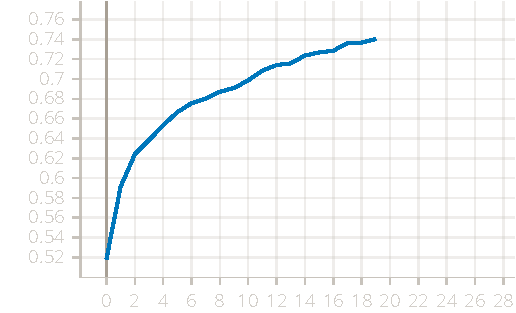
\includegraphics[width=\textwidth]{img/F1_train.pdf}
        \caption{F1-Score (Entrenamiento)}
        \label{fig:f1_train}
    \end{subfigure}
    \hfill
    \begin{subfigure}{0.48\textwidth}
        \centering
        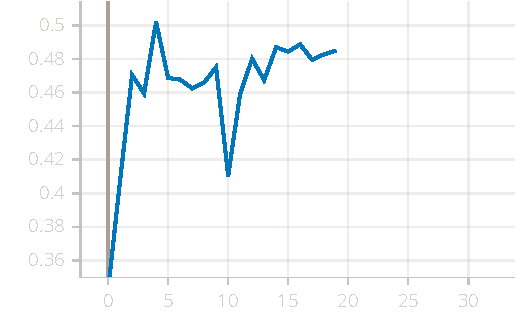
\includegraphics[width=\textwidth]{img/F1_val.pdf}
        \caption{F1-Score (Validación)}
        \label{fig:f1_val}
    \end{subfigure}
    
    \vspace{0.5cm}
    
    \begin{subfigure}{0.48\textwidth}
        \centering
        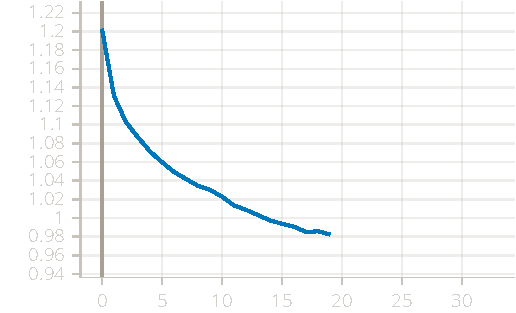
\includegraphics[width=\textwidth]{img/Loss_train.pdf}
        \caption{Loss (Entrenamiento)}
        \label{fig:loss_train}
    \end{subfigure}
    \hfill
    \begin{subfigure}{0.48\textwidth}
        \centering
        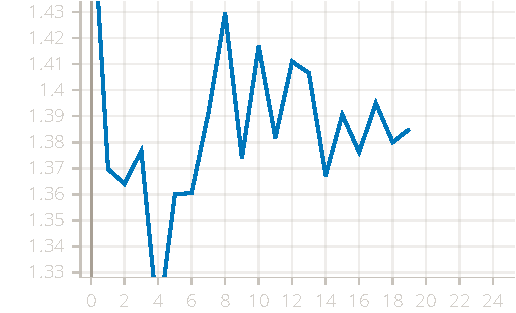
\includegraphics[width=\textwidth]{img/Loss_val.pdf}
        \caption{Loss (Validación)}
        \label{fig:loss_val}
    \end{subfigure}
    
    \caption{Curvas de aprendizaje del modelo. Arriba: Evolución del \textit{Macro F1-score}. Abajo: Evolución de la función de pérdida (\texttt{CrossEntropyLoss}). Se observa el comportamiento en los conjuntos de entrenamiento y validación.}
    \label{fig:metricas_grid}
\end{figure}

\begin{figure}[hbt!]
    \centering
    \begin{subfigure}{0.48\textwidth}
        \centering
        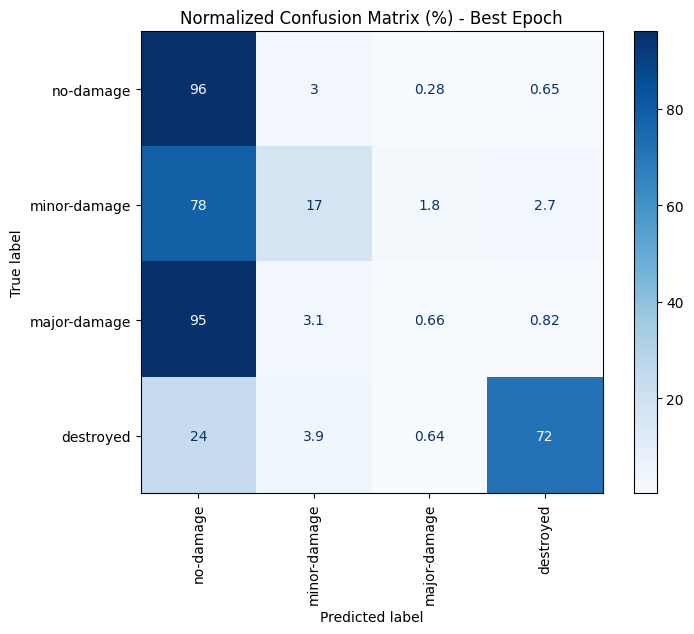
\includegraphics[width=\textwidth]{img/best_confusion_matrix.png}
        \caption{Modelo CustomNet}
        \label{fig:cm_custom}
    \end{subfigure}
    \hfill
    \begin{subfigure}{0.48\textwidth}
        \centering
        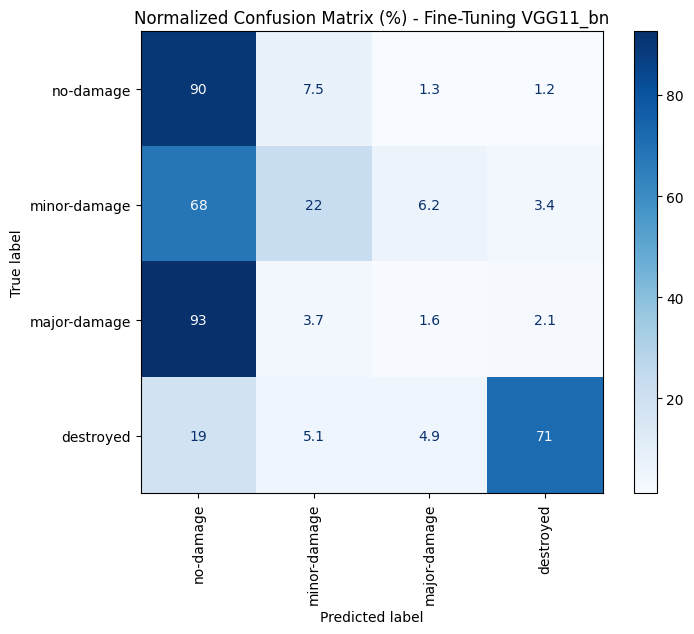
\includegraphics[width=\textwidth]{img/best_ft_confusion_matrix.png}
        \caption{Modelo Fine-Tuning (\texttt{VGG11\_bn})}
        \label{fig:cm_ft}
    \end{subfigure}
    
    \caption{Comparativa de matrices de confusión evaluadas en el conjunto de validación. A la izquierda, el modelo diseñado desde cero. A la derecha, el modelo pre-entrenado con \textit{fine-tuning}.}
    \label{fig:confusion_matrices}
\end{figure}

\section{Conclusiones}

El análisis crítico del proyecto revela que el éxito en esta tarea, dadas las condiciones tan peculiares de la base de datos, no recae en la profundidad de la red, sino en el manejo de otros aspectos. La técnica con mayor impacto positivo fue la combinación de un modelo estilo VGG con \texttt{AdamW}, \texttt{CrossEntropyLoss} y \textit{label smoothing}, \texttt{CosineAnnealingLR} y transformaciones básicas. Es necesario añadir que, durante la etapa de búsqueda, se encontró informacion relacionada con que entrenar la red usando técnicas más avanzadas como modelos de atención, o incluso entrenar la red usando imágenes pre y post desastre, aumentarían el desempeño.

\end{document}
